%The document's type
\documentclass[a4paper,11pt]{article}

%Additionnal packages
\usepackage{color}
\usepackage[latin1]{inputenc}
\usepackage[T1]{fontenc}
\usepackage[english]{babel}
\usepackage{graphicx}
\usepackage{hyperref}
\usepackage{indentfirst}


%%%%%%%%%% Start TeXmacs macros
\newcommand{\tmbsl}{\ensuremath{\backslash}}
\newcommand{\tmem}[1]{{\em #1\/}}
\newcommand{\tmstrong}[1]{\textbf{#1}}
\newcommand{\tmtexttt}[1]{{\ttfamily{#1}}}
\definecolor{grey}{rgb}{0.75,0.75,0.75}
\definecolor{orange}{rgb}{1.0,0.5,0.5}
\definecolor{brown}{rgb}{0.5,0.25,0.0}
\definecolor{pink}{rgb}{1.0,0.5,0.5}
%%%%%%%%%% End TeXmacs macros

\title{Market microstructure simulation library Marketsim\\Overview}
\author{Anton Kolotaev}

\begin{document}

\maketitle

\tableofcontents



















\newpage

\section{Introduction}
Last years financial market microstructure attracts more and more
attention due to its potential capability to explain some macroscopic
phenomena like liquidity crisis, herd behaviour that were observed during
recent crises. Researchers in this field need a simulation tool that would
support them in their theoretical studies. This tool would take into
account in exhaustive and precise manner market rules: how orders are sent to the market,
how they are matched, how information is propagated.

An architecture of this tool should allow to model any behaviour of market
agents, i.e. to be very flexible in trading strategies definition. It might be
used to study impact on market caused by changing tick size, introducing
a new order type, adding a new order matching rule.
Used-friendliness is also very important quality expected from the the simulator. 
Since a typical simulation model is composed of
many hundreds and thousands blocks, it is very important to provide
a simple way for user to tell how a behaviour wanted differs from the
default one. 
As simulation models grow their simulation time become an important issue. A good simulator shall 
have different levels of optimisation: for experiments that run shortly it is reasonable not to spend time for optimisations while simulations for long-running experiments should be well optimised.

Representing a simulation model as a network of modules communicating
by messages is a widely accepted practice for discrete-event systems (e.g.
Omnet++ or ns-2 frameworks to simulate telecommunication networks).
Modules may have parameters thus allowing to adjust their behaviour.
We will distinguish two sorts of modules:
\begin{enumerate}
\item \emph{Simple modules} provide functionality which is considered elementary
(and there is no reason to reuse part of it to implement other
modules).
\item \emph{Compound modules} combine together other modules in some way
and define their parameters based on its own parameters. Compound
module behaviour is just a composition of its constituting modules
behaviours.
\end{enumerate}
The following figure illustrates a modular design for a crossing averages trading strategy.

\centerline{\includegraphics[width=1\linewidth]{talks/graph.png}}

As modular design evolves modules become smaller but code composing them gets more complicated. 
If this code was written in an object-oriented language it would consist completely from object constructor calls. Since only a small subset of a general purpose language is needed we may introduce a domain-specific language (DSL) obtaining the following profits:

\begin{enumerate}
\item \textbf{\textit{Syntax}}. We may design the DSL so its syntax describes very well domain specific abstractions and diminish syntax noise typical for solutions based on general-purpose language use.
\item \textbf{\textit{Error checking}}. A DSL compiler can detect incorrect parameter values as soon as possible thus shortening simulation development cycle and facilitating refactorings.
\item \textbf{\textit{Multiple target languages}}. A DSL can be compiled into different languages: e.g. into Python to provide fast start-up and into C++ to have highly optimized fast simulations. A new target language introduced, only simple modules need to be re-written into it; compound modules will be ported automatically.
  \item \textbf{\textit{IDE support}}. Modern IDEs like Eclipse, Intellij IDEA allow writing plug-ins that provide smart syntax highlighting, auto-completion and error checking on-the-fly for user-defined DSLs.
  \item \textbf{\textit{High-level optimizations}} are easier to implement. 
  \item \textbf{\textit{Safety}}. In case of a web interface a code written by a user in DSL can be safely run on a server. If model code was written in a general-purpose language significant efforts would be required to run it safely on server without considerable performance overhead.
\end{enumerate}

A simulation library must have a very modular design in order to provide a high level of flexibility to the user. This requirement comes from the original purpose of a simulation as a testbed for experiments with different models and parameters.

In object-oriented languages various sorts of dynamic method invocation (virtual functions or dispatch methods) are used for module parametrisation. The dynamic nature of the calls hinders the compiler in performing many useful optimisations. Finer grain modularity leads to smaller objects, and thus to a higher overhead, something known as abstraction penalty.

The C++ provides a solution to avoid this abstraction penalty while keeping modularity at high level: static polymorphism via class and function templates. However, such methods require expertise in C++ programming thus limiting the potential user base.

In order to achieve high performance (comparable to hand written C code), C++ template instantiations can be generated automatically from an abstract simulation model representation via an object graph. Only simple modules need to be re-implemented in C++; compound modules are represented already in an abstract way and C++ code for them can be generated automatically.

\section{Strategy Definition Language}\label{SDL}

\subsection{Functions}

Essentially, a program in Strategy Definition Language (SDL) consists of function declarations and all other constructs desugar into function declaration at compile time.

Functions in Strategy Definition Language correspond to simple and compound modules in a simulation model. Functions have parameters which are used to generate module fields. Every parameter is defined by an unique name, a type and an optional default value. Parameter type tells what kind of values may be assigned to this field. Conceptually, a "function" declaration defines a term with a constructor provided (like case classes in Scala).

Simple modules represent some functionality which is considered as elementary and they are implemented in target language (like Python). Functions for simple modules (intrinsic functions) don't have body but they must be decorated by an annotation telling where its implementation in the target language should be taken from (e.g. \texttt{\@python.intrinsic(\"\_Class\_Impl\")}).

For example, an observable that adds a lag to an observable data source so \texttt{Lagged(x, dt)(t0+dt) = x(t0)} could be declared as

\begin{verbatim}
@python.intrinsic("observable.lagged.Lagged_Impl")
def Lagged (/** observable data source */   
            source    = const (1.),
            /** lag size */
            timeframe = 10.0) : IObservable[Float]
\end{verbatim}

Compound modules are compositions of other modules and can be completely generated from a high level description at Strategy Definition Language. Functions describing them must have a body defining how they are composed.

Functions are assigned types and these types allows modules to be used as parameters for other modules.

\texttt{LogReturns} function may serve as a good example of a compound module: it is just a composition of a \texttt{Log}, \texttt{Lagged} and \texttt{/} modules.

\begin{verbatim}
def LogReturns(/** observable data source */   
               x = const(1.),
               /** lag size */                
               timeframe   = 10.0)

        =  Log(x / x~>Lagged(timeframe))
\end{verbatim}

All methods can be considered as extension methods of their first argument. 

Thus, \texttt{x$\sim$>Lagged(dt)} is equivalent to \texttt{.observable.Lagged(x, dt)}.

Types for input arguments are inferred automatically from their initializers and for the "return" value - from the function body.

\subsection{Types}

The Strategy Definition Language aims to introduce a strict static type system in order to prevent errors as soon as possible. Though this task hasn't been completely accomplished yet and sometimes a user has to do explicit downcasts, the type system is evolving in order to avoid them.


\subparagraph{Predefined types}

\begin{itemize}
\itemsep1pt\parskip0pt\parsep0pt
\item
  \textbf{Unit type}: \texttt{()}
\item
  \textbf{Simple types}: \texttt{Float}, \texttt{Int} etc.
\item
  \textbf{Tuple types}: \texttt{(t1, t2, ... tn)} where \texttt{ti} are
  other types (n \textgreater{}= 2 is implied, for n = 0 a unit type
  should be used, and for n = 1 a simple type should be used). In future
  it might be useful to consider unit type as a particular case of a
  tuple type.
\item
  \textbf{Function types}: \texttt{args\_type =\textgreater{} ret\_type}
  where \texttt{arg\_type} may be a unit type, simple type, tuple type
  or another function type
\end{itemize}

Some simple types must be declared by the user and the following code
must appear in a model description (it is done for readability reasons
in order to show what types are defined):

\begin{verbatim}
type Any

type Float
type Int : Float
type Boolean
type String

type Optional[T]
type List[T]
\end{verbatim}

\subparagraph{Generic types.}


User defined types may have generic parameters that are used in their
definition. Contravariance rules are applied for function type
arguments: \texttt{T\,\textless{}:\,U} implies
\texttt{U\,=\textgreater{}\,X\,\textless{}:\,T\,=\textgreater{}\,X}. For all
other cases covariance is used: \texttt{T\,\textless{}:\,U} implies
\texttt{List{[}T{]}\,\textless{}:\,List{[}U{]}} and
\texttt{T\,\textless{}:\,U} implies
\texttt{()\,=\textgreater{}\,T\,\textless{}:\,()\,=\textgreater{}\,U}. (We use
notation \texttt{T\,\textless{}:\,U} to show that type \texttt{T} can be
casted to type \texttt{U})

\subparagraph{Type aliases} behave like \texttt{typedef} in C++ and introduce a handy
shortcut for another type. For example,

\begin{verbatim}
type IFunction[T] = () => T
\end{verbatim}

Alias for a type equals to it. It implies that in the following code

\begin{verbatim}
def f() : () => Float
def g() : IFunction[Float]
\end{verbatim}

functions \texttt{f} and \texttt{g} have the same type.

\subparagraph{User-defined types.}


A user may define own types. These types may inherit from other types:

\begin{verbatim}
type IObservable[T] : IFunction[T], IEvent
\end{verbatim}

In this sample type \texttt{IObservable{[}Float{]}} may be used in any
place where \texttt{IFunction{[}Float{]}} or \texttt{IEvent} is expected
(but not vice versa).

\subparagraph{Special types.}


Type \texttt{Any} is an implicit super type for any type, i.e. any type
casts to \texttt{Any}. For example, \texttt{IObservable{[}Float{]}}
casts to \texttt{IObservable{[}Any{]}}.

Type \texttt{Optional{[}T{]}} appears at function declarations having
default arguments. Any type \texttt{T} casts to
\texttt{Optional{[}T{]}}.

Lists can be constructed using following syntax:
\texttt{{[}e1,e2,...,en{]}} where \texttt{ei} are some expressions and
they have type \texttt{List{[}T{]}} where \texttt{T} is the bottommost
type all \texttt{ei} can be casted to.

Type \texttt{Nothing} is the bottommost type so it can be casted to any
type. For the moment it appears only when an empty list is declared so
literal \texttt{{[}{]}} has type \texttt{List{[}Nothing{]}} and can be
casted to \texttt{List{[}T{]}} for any \texttt{T}.

\subsection{Classes}\label{classes}

Classes are syntax sugar for a type declaration, a constructor function and member accessors. They allow to get rid of excessive enumerations of similar parameter lists.

For example, Moving Average Convergence/Divergence, its signal and histograms are closely connected and share \texttt{slow} and \texttt{fast} attributes.

\begin{verbatim}
type macd(/** source */       source = .const(1.),
          /** long period */  slow = 26.0,
          /** short period */ fast = 12.0)
{
    /**
     *  Moving average convergence/divergence
     */
    def Value = source~>EW(2./(fast+1))~>Avg -
                source~>EW(2./(slow+1))~>Avg

    /**
      *  Moving average convergence/divergence signal
      */
    def Signal(/** signal period */        
               timeframe = 9.0,
               /** discretization step */   
               step = 1.0)

    = Value~>OnEveryDt(step)~>EW(2/(timeframe+1))~>Avg

    /**
      *  Moving average convergence/divergence histogram
      */
    def Histogram(/** signal period */
                  timeframe = 9.0,
                  /** discretization step */   
                  step = 1.0)

        = Value - Signal(timeframe, step)
}
\end{verbatim}

The previous definition is de-sugared at typing stage into

\begin{itemize}
\item Type declaration
\begin{verbatim}
type macd
\end{verbatim}
\item Type constructor 
\begin{verbatim}
def macd(/** source */       source = .const(1.),
         /** long period */  slow = 26.0,
         /** short period */ fast = 12.0) : macd
\end{verbatim}
\item Accessor methods
\begin{verbatim}
def Source(x = macd()) : IObservable[Float]
def Slow(x = macd()) : Float
def Fast(x = macd()) : Float
\end{verbatim}
\item Methods rewritten as free functions
\begin{verbatim}
def Value(x = macd()) =
   x~>source~>EW(2./(x~>fast+1))~>Avg -
   x~>source~>EW(2./(x~>slow+1))~>Avg

def Signal(x = macd(),        
           timeframe = 9.0,
           step = 1.0) = 
    x~>Value~>OnEveryDt(x~>step)~>EW(2/(x~>timeframe+1))~>Avg

def Histogram(x = macd(),
              timeframe = 9.0,
              step = 1.0)

    = x~>Value - Signal(x~>timeframe, x~>step)
\end{verbatim}
\end{itemize}

For better readability, nested classes language feature could be implemented in the future and it would allow to share \texttt{timeframe} and \texttt{step} parameters between \texttt{Signal} and \texttt{Histogram} in the previous example.

Class inheritance serve to share parts of common implementation between classes. All methods are treated as "virtual" to stimulate code re-use.

For example, there are different kind of moving averages (simple moving window, cumulative, exponentially weighted). They have different implementations but variance and standard deviation can be implemented in the same way for all of them.

First, we factor out common implementation where we assume that all derived classes define method \texttt{Avg}

\begin{verbatim}
abstract type IStatDomain(source = .const(0.))
{
    /** Variance */
    def Var = source~>Sqrt~>Avg - source~>Avg~>Sqrt
    
    /** Standard deviation  */
    def StdDev = Var~>Sqrt

    /** Relative standard deviation */
    def RelStdDev = (source - Avg) / StdDev
}
\end{verbatim}

\textit{Note: in order to avoid numerical precision losses \texttt{Var} is implemented intrinsically for every kind of moving average}

Then, we declare how concrete classes differ from the common implementation

\begin{verbatim}
type Cumulative() : IStatDomain
{
    /** Cumulative average */
    @python.intrinsic("moments.cma.CMA_Impl")
    def Avg : IDifferentiable
}

type EW(alpha = 0.015) : IStatDomain
{
    /** Exponentially weighted moving average */
    @python.intrinsic("moments.ewma.EWMA_Impl")
    def Avg : IDifferentiable
}

type Moving(timeframe = 100.) : IStatDomain
{
    /** Simple moving average */
    @python.intrinsic("moments.ma.MA_Impl")
    def Avg : IDifferentiable
}
\end{verbatim}

\subsection{Packages}

Packages are used to group functions and types. They can be nested. Attributes are inherited from enclosing package. Anonymous packages are used to assign same attributes to a group of functions without introducing a new name scope.

\begin{verbatim}
@X = "X"
@Y = "Y"
package A.B {
    @X = "Xa"
    def f() => Float
    
    @X = "Xb"
    package {
        def g() => Float
        def h() => Float
    }
}
\end{verbatim}

In this sample \texttt{.A.B.f} will have attributes \texttt{X == "Xa", Y == "Y"} and \texttt{.A.B.g} and \texttt{.A.B.h} will have attributes \texttt{X == "Xb", Y == "Y"}

\subsection{Example: Relative Strength Index strategy}\label{RSI}

First, we define observables corresponding to positive and negative movements of some process:

\begin{verbatim}
def UpMovements(/** observable data source */   
                source = const (1.),
                /** lag size */                
                timeframe = 10.0)

   = Max(0.0, source - source~>Lagged(timeframe))

def DownMovements(/** observable data source */   
                  source = const (1.),
                  /** lag size */                 
                  timeframe = 10.0)

   = Max(0.0, source~>Lagged(timeframe) - source)
\end{verbatim}

Then we may define Relative Strength Index:

\begin{verbatim}
type RSI(/** observable data source */   
         source      = .const (1.),
         /** lag size */                 
         timeframe   = 10.0,
         /** alpha parameter for EWMA */ 
         alpha       = 0.015)
{
    /** Absolute value for Relative Strength Index */
    def Raw =
        source~>UpMovements  (timeframe)~>EW(alpha)~>Avg /
        source~>DownMovements(timeframe)~>EW(alpha)~>Avg

    def Value = 100.0 - 100.0 / (1.0 + Raw)
}
\end{verbatim}

Our strategy will be a particular case of  \texttt{DesiredPosition} strategy: it believes that the trader position should be equal to some time-dependent value and in some moments of time it calculates difference between the actual position and the desired one and sends a market order to compensate this difference. 

\begin{verbatim}
abstract type DesiredPositionStrategy
{
    def Position = 
        DesiredPosition - trader~>Position - trader~>PendingVolume

    def Strategy(/** order factory function */
                 orderFactory = order.signedVolume.MarketSigned()) 
        = (orderFactory(Position))~>Strategy
}
\end{verbatim}

It expects that its descendants provide fields \texttt{DesiredPosition} and \texttt{trader}.\texttt{RSI\_linear} strategy is inherited from \texttt{DesiredPositionStrategy} and defines these fields:

\begin{verbatim}
/**
 *  Strategy believing that trader position should
 *  be proportional to 50 - RSI(asset)
 */
type RSI_linear(
        /** alpha parameter for exponentially moving averages of 
         * up movements and down movements */
        alpha = 1./14.,
        /** observable scaling function that maps
          *  RSI deviation from 50 to the desired position */
        k = .const(-0.04),
        /** lag for calculating up and down movements */
        timeframe = 1.,
        /** trader in question */
        trader = .trader.SingleProxy()) : DesiredPositionStrategy
{
    def DesiredPosition = (50. -
        trader~>Orderbook~>MidPrice
                         ~>RSI(timeframe, alpha)
                         ~>Value
                         ~>OnEveryDt(1.0)) * k
}
\end{verbatim}
\section{User interfaces}

For the moment the simulator has a web-based graphical user interface and also can be scripted in Python. The first approach is easier for new users while the latter one gives more control over simulation.

Latest public version of the simulator can be downloaded from
\url{https://github.com/fiquant/marketsimulator/releases}. Project documentation can be found at \url{https://github.com/fiquant/marketsimulator/README.md}

The market simulator can be deployed on some server and a user may use a web interface to it to set up model parameters and run the simulation. 

\centerline{\includegraphics[width=1\linewidth]{Figures/web/traders.png}}

Simulation results are rendered in form of graphs. Following figure shows "volume levels" showing  how many orders in an orderbook have price better than a given one.

\centerline{\includegraphics[width=1\linewidth]{Figures/web/volume-levels.png}}

Also a user may create scripts describing a simulation, run them in the simulator and the results will be rendered using Veusz software (in principle, it quite easy to plug in another means of visualization).

\centerline{\includegraphics[width=1\linewidth]{Figures/veusz/dependency.png}}

\section{Evolution of the simulator}\label{evolution-of-the-simulator}

\begin{enumerate}
\def\labelenumi{\arabic{enumi}.}
\itemsep1pt\parskip0pt\parsep0pt
\item
  Initial
  \href{http://sourceforge.net/p/marketsimulator/svn/HEAD/tree/Simulator/}{C++
  version} was developed in 2009-2011 by Riadh Zaatour.
\item
  In order to improve its extensibility and performance the simulator
  was \href{https://github.com/antonkolotaev/v2}{rewritten} using C++
  template metaprogramming techniques by
  \href{https://github.com/antonkolotaev}{Anton Kolotaev} in 2012.
  Python bindings to it were implemented using Boost.Python.
  Unfortunately the price for providing high extensibility with no
  overhead was quite high: in order to use it a proficiency in C++
  template metaprogramming was required.
\item
  A new pure Python version was designed and developed in 2013 by
  \href{https://github.com/antonkolotaev}{Anton Kolotaev}. The main idea
  of its design is representation of a simulation model as a composition
  of simple and compound modules. 
\item
  A web interface allowing to set up model parameters and launch the
  simulation was developed by
  \href{https://github.com/antonkolotaev}{Anton Kolotaev} in JavaScript
  using \href{http://knockoutjs.com/}{KnockoutJs} as MVVM framework and
  \href{http://www.highcharts.com/products/highstock}{Highstock} as
  graph visualisation library.
\item
  \href{https://github.com/koalainparis}{Karol Podkanski} has
  implemented number of trading strategies and indicators during his
  internship at summer 2013 (initial implementation for Relative
  Strength Index, Bollinger Bands, Market Data and Market Maker
  strategies, StopLoss meta order, statistical indicators and adaptors
  for existing statistics packages:
  \href{http://pandas.pydata.org/}{pandas} and
  \href{http://ta-lib.org/}{ta-lib})
\end{enumerate}

A dedicated language for module abstract description is developed.
A compiler from this language generates Python implementations for
compound modules and also all meta information about available modules
needed for the Web interface. 

\section{Discrete event simulation
components}\label{discrete-event-simulation-components}

The main class for every discrete event simulation system is a scheduler
that maintains a set of actions to fulfill in future and launches them
according their action times: from the older ones to newer ones. The
scheduler in the simulator is implemented as a heap data structure in
order to perform frequent operations very fast. A classical heap allows
inserts into at O(logN), extracting the best element at O(logN) and
accessing to the best element at O(1). A bucket-based implementation may
be introduced in order to improve performance provided that the
distribution of event times should is beforehand.

\texttt{Scheduler} class provides following interface:
\begin{verbatim}
class Scheduler(object):

    # cleans up event queue and resets simulation time to 0
    def reset(self)

    @property
    def currentTime(self)

    # schedules an event given by 'handler' to be launched at 'actionTime'
    def schedule(self, actionTime, handler)

    # schedules an event given by 'handler' to be launched after 'dt' from now
    def scheduleAfter(self, dt, handler):
        self.schedule(self.currentTime + dt, handler)

    # runs 'handler' asynchronously
    def async(self, handler):
        self.scheduleAfter(0, handler)

    # Launches all events with action time in range [currentTime, limitTime)
    # in order of their action time and arrival order
    def workTill(self, limitTime)

    # Makes the scheduler work 'dt' moments of time more
    def advance(self, dt)
        self.workTill(self.currentTime + dt)
\end{verbatim}

In order to schedule an event a user should use \texttt{schedule} or
\texttt{scheduleAfter} methods passing there an event handler which
should be given as a callable object (a function, a method, a lambda
expression or an object exposing \texttt{\_\_call\_\_} method).

Methods \texttt{workTill} and \texttt{advance} advance model time
calling event handlers in order of their action times. If two events
have same action time it is garanteed that the event scheduled first
will be executed first. 

Components willing to have an access to the scheduler should acquire a
reference to it at binding time:

\begin{verbatim}
def bind(self, ctx):
    self._scheduler = ctx.world
\end{verbatim}


\section{Events, functions and
observables}\label{events-functions-and-observables}

\subsection{Events}\label{events}
\textbf{Events} in the simultator are conceptually close to events in
C\# or to \texttt{boost::signal} in C++. Listeners can be
subscribed for event notification using \texttt{+=} operator and
unsubscribed with \texttt{-=} operator. A listener should be a callable
object that accepts a single argument - the source of the event (it
allows not to store an event source in the listener and also use a
single listener for several event sources at the same time).

\subsection{Event subscription}\label{event-subscription}

Since event subscription is often done at binding time and unadvising
should be done at dispose time \texttt{event.subscribe} helper function
was introduced to manage event subscription declaratively:

\begin{verbatim}
class ProgressPrinter(object):

  def __init__(self):
    event.subscribe(event.Every(ops.constant(10)), # event source to subscribe to
                    _(self)._wakeUp,               # event listener
                    self)

  def _wakeUp(self, _):
    print '.'   # prints . every 10 units of time
\end{verbatim}

\subsection{Event helpers}\label{event-helpers}

\texttt{event.After} and \texttt{event.Every} are used to represent a
single and a repeating action

\texttt{event.Array} is used when several event sources are to be
represented as a single event. For example,

\begin{verbatim}
event.Array([BestPrice(Asks(orderbook)), BestPrice(Bids(orderbook))])
\end{verbatim}

fires an event once bid or ask of \texttt{orderbook} has changed.

\subsection{Filtered events}\label{filtered-events}

Sometimes an event source (for example, price of an asset) has hundreds
subscribers who check whether the event source is less or greater than some
value. In order to avoid excessive calls \texttt{event.LessThan} and
\texttt{event.GreaterThan} classes are introduced. Event sources detect
objects of these types and store them sorted in order to lookup relevant
listeners very quickly. For example,

\begin{verbatim}
observable.MidPrice(orderbook) += event.LessThan(100, listener)
\end{verbatim}

will call \texttt{listener} only if mid-price of the asset is less than
100.

\subsection{Functions and observables}\label{functions-and-observables}

\begin{description}
\item[Function]
Object with overloaded \texttt{\_\_call\_\_} operator that accepts no
arguments and returns a value of type \texttt{T}. Further we will refer
to the type of a function as \texttt{() -\textgreater{} T} or
\texttt{IFunction}.
\item[Observable]
Function notifying listeners about its value changes. Only piecewise
constant functions should be considered as observables. An arbitrary
function can transformed into observable by means of
\texttt{observable.OnEveryDt(dt, func)}.
\end{description}

Conceptually an observable could be defined as

\begin{verbatim}
class IObservable[T] (IFunction[T], IEvent): ...
\end{verbatim}
\subsection{Basic observables}\label{basic-observables}

\begin{itemize}
\item
  \texttt{Constant{[}T{]}} / \texttt{None{[}T{]}} represent typed
  constant value or \texttt{None} value
\item
  \emph{Arithmetic operations} (\texttt{Sum}, \texttt{Sub}, \texttt{Product},
  \texttt{Div}, \texttt{Mod}). If both arguments of the operation are
  observable the operation fires events about its value change and thus
  becomes an event itself. Functions overload operations \texttt{+},
  \texttt{-}, \texttt{*}, \texttt{-}, \texttt{\%} so they construct
  respective objects. For example,
  \begin{verbatim}
(observable.AskPrice(orderbook) + observable.BidPrice(orderbook)) / 2  
  \end{verbatim}
  creates an observable that notifies about every change of the
  mid-price.
\item
  \emph{Logic operations} (\texttt{Equal{[}T{]}}, \texttt{NotEqual{[}T{]}},
  \texttt{Less{[}T{]}}, \texttt{Greater{[}T{]}},
  \texttt{GreaterEqual{[}T{]}}, \texttt{LessEqual{[}T{]}}). If both
  arguments of the operation are observable the operation fires events
  about its value change and thus becomes an event itself. Functions
  overload operations \texttt{==}, \texttt{!=}, \texttt{\textgreater{}=}, \texttt{\textgreater{}}, \texttt{\textless{}}, \texttt{\textless{}=} so they construct
  respective objects. These operations inherit from
  \texttt{IFunction{[}bool{]}}/\texttt{IObservable{[}bool{]}} and have
  overloaded indexing operator that constructs \texttt{Condition{[}T{]}}
  object and it allows to write if-then-else expressions like:

\begin{verbatim}
# randomly chooses either Side.Buy or Side.Sell
(math.random.uniform(0.,1.) < 0.5)[ 
    ops.constant(Side.Buy), ops.constant(Side.Sell) 
]
\end{verbatim}
\item
  Functions from standard \texttt{math} module: \texttt{Atan},
  \texttt{Pow} etc
\item
  Random distributions from \texttt{random} module: \texttt{uniform},
  \texttt{lognormvariate}, \texttt{expovariate} etc.
\item
  \texttt{Lagged}: returns function values with some lag

\begin{verbatim}
def Min(x = constant(1.), y = constant(1.)) = if x < y then x else y
def Max(x = constant(1.), y = constant(1.)) = if x > y then x else y

def Sqr(x = constant(1.)) = x*x
\end{verbatim}

\item
  \texttt{Quotes}: downloads external historical data
  
\item \emph{Current simulation time.}
For example,

\begin{verbatim}
(observable.CurrentTime() < 200)[Side.Sell, Side.Buy]
\end{verbatim}

returns \texttt{Side.Sell} if simulation time is less than 200 and
\texttt{Side.Buy} otherwise
\end{itemize}

There are also statistics related functions,
functions of orderbooks and of traders.

\section{Statistics}\label{statistics}

Statistical functions operate on paths of function values and in general
case it requires storing the function history and recalculating
statistics each time. Every recalculation has at least O(M) time
complexity where M is number of points involved and thus it is quite
time consuming.

Many statistical packages (like \href{http://pandas.pydata.org/}{pandas}
and \href{http://ta-lib.org/}{ta-lib}) provide a lot of useful functions
that work on time series and in order to facilate interoperability with
these libraries the market simulator provide handful adapters.

In some cases (moving average, moving variance etc) it is possible to
introduce an incremental version that make every update in constant time
and thus works much faster.

\subsection{Moving average}\label{moving-average}

\begin{itemize}
\itemsep1pt\parskip0pt\parsep0pt
\item
  cumulative: \texttt{math.Cumulative.Avg}
\item
  simple moving: \texttt{math.Moving(timeframe).Avg}
\item
  exponentially weighted: \texttt{math.EW(alpha).Avg}
\end{itemize}

\centerline{\includegraphics[width=1\linewidth]{Figures/web/averages.png}}

\subsection{Moving average
convergence/divergence}\label{moving-average-convergencedivergence}

Having defined moving average we may introduce
\href{http://en.wikipedia.org/wiki/MACD}{moving average
convergence/divergence}, its signal and histogram. 
\begin{verbatim}
MACD(x, slow, fast) ::= 
    EWMA(x, 2./(fast+1)) - EWMA(x, 2./(slow+1))

MACD_signal(x, slow, fast, timeframe) ::= 
    EWMA(MACD(x, slow, fast), 2/(timeframe+1))

MACD_histogram(x, slow, fast, timeframe) ::= 
    MACD(x,slow,fast) - MACD_signal(x,slow, fast, timeframe)
\end{verbatim}

\centerline{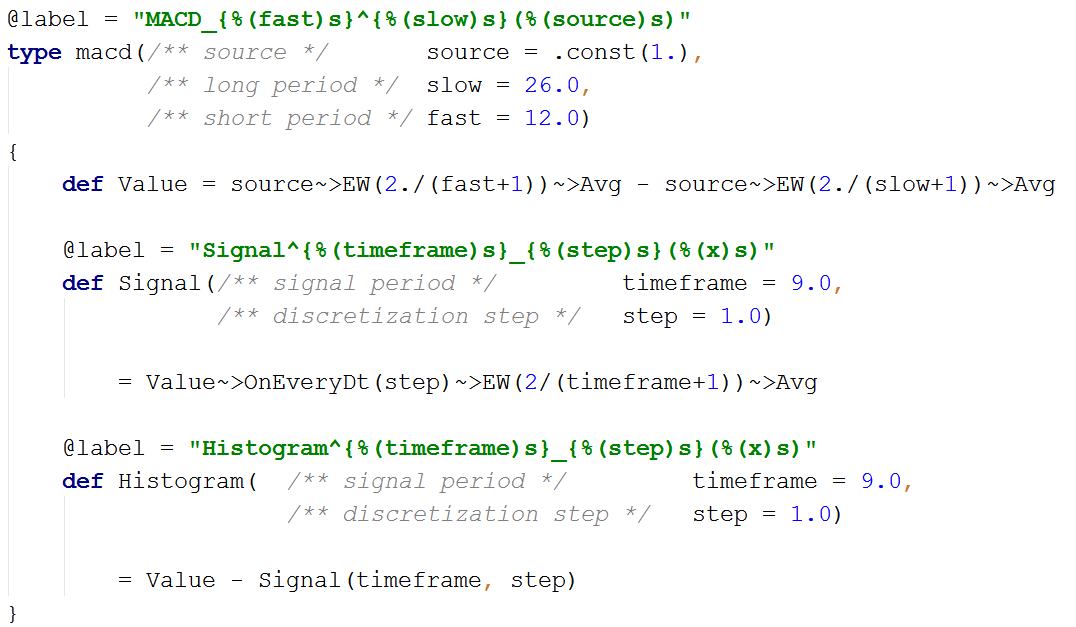
\includegraphics[width=1\linewidth]{Figures/web/macd.png}}

\subsection{Moving variance and standard deviation}\label{moving-variance}

\begin{itemize}
\itemsep1pt\parskip0pt\parsep0pt
\item
  cumulative: \texttt{math.Cumulative.Var} and \texttt{math.Cumulative.StdDev}
\item
  moving: \texttt{math.Moving(timeframe).Var} and \texttt{math.Moving(timeframe).StdDev}
\item
  exponentially weighted: \texttt{math.EW(alpha).Var} and \texttt{math.EW(alpha).StdDev}
\end{itemize}
Variances could be implemented via averages but it looses precision so they
are implemented as simple modules

\begin{verbatim}
Var(x) ::= Avg(Sqr(x)) - Sqr(Avg(x))
\end{verbatim}


\subsection{Bollinger bands}\label{bollinger-bands}

Having moving averages and variances it is possible to find
\href{http://en.wikipedia.org/wiki/Bollinger_Bands}{bollinger bands}:

\begin{verbatim}
Bollinger_Hi(x) ::= Mean(x) + 2*StdDev(x)
Bollinger_Lo(x) ::= Mean(x) - 2*StdDev(x)
\end{verbatim}

\centerline{\includegraphics[width=1\linewidth]{Figures/web/bollinger_bands.png}}

\subsection{Relative strength index}\label{relative-strength-index}

An observable returning values of a function with some lag
(\texttt{Lagged}) allows easily implement
\href{http://en.wikipedia.org/wiki/Relative_strength_index}{relative
strength index}. Implementation can be found here: \ref{RSI}.

\centerline{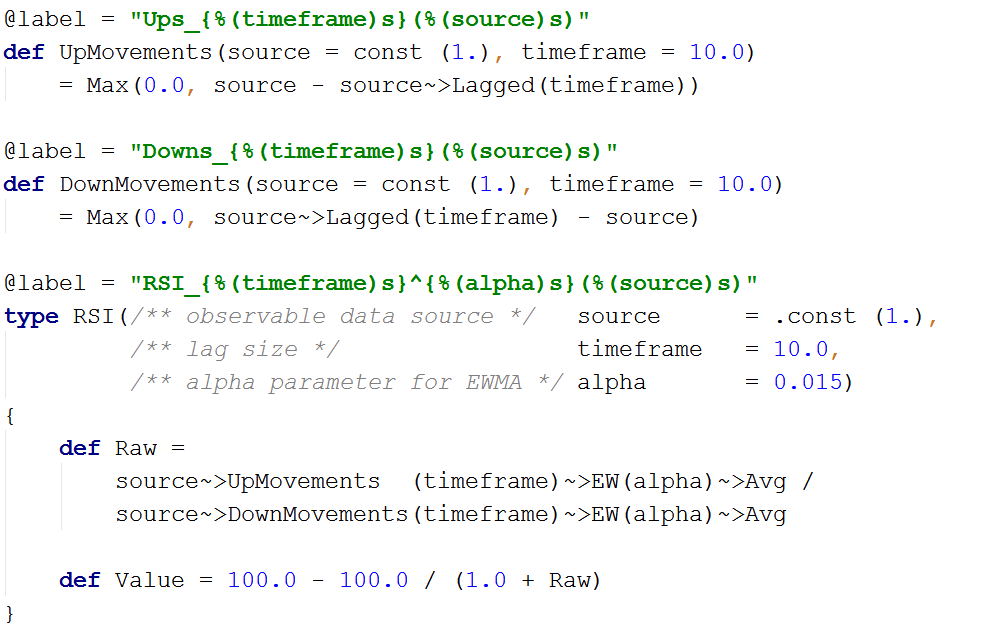
\includegraphics[width=1\linewidth]{Figures/web/rsi.png}}

\subsection{Moving minimum and maximum}\label{moving-minimum-and-maximum}
\centerline{\includegraphics[width=1\linewidth]{Figures/web/minmax.png}}

\section{Elementary orders, their factories and
requests}\label{elementary-orders-their-factories-and-requests}

Traders send orders to a market. There are two basic kinds of orders:

\begin{itemize}
\itemsep1pt\parskip0pt\parsep0pt
\item
  \textbf{Market orders} ask to buy or to sell some asset at any price.
\item
  \textbf{Limit orders} ask to buy or to sell some asset at price better
  than some limit price. If a limit order is not competely fulfilled it
  remains in an order book waiting to be matched with another order.
\end{itemize}

An order book processes market and limit orders but keeps persistently
only limit ones. Limit orders can be cancelled by sending cancel
request.

From trader point of view there can be other order types like
Iceberg order but from order book
perspective it is just a sequence of basic orders and requests. They
will be covered at meta orders section.

Besides basic orders there are also requests: order cancellation
request, request to estimate market impact of a trade etc. Their
interface differs a lot from orders' interface that's why they are put
into a separate group.

\subsection{Market and limit orders}\label{market-and-limit-orders}

Market and limit orders (and some meta orders) derive from a common base
class that provides some basic functionality:

\begin{itemize}
\itemsep1pt\parskip0pt\parsep0pt
\item
  matched/unmatched volume management: \texttt{volumeUnmatched}, \texttt{empty} etc
\item
  storing a cancellation flag: \texttt{cancelled}, \texttt{cancel}
\item
  keeping a reference to the order's owner: \texttt{owner}
\end{itemize}


Classes \texttt{order.Market} and \texttt{order.Limit} derive from this
class and define method \texttt{processIn(orderbook)} which defines how
the order should be processed in an orderbook.

When the order is matched against another order it calls
\texttt{onMatchedWith} method of the \texttt{owner} passing volume and
price at which the trade was done.

If an order is cancelled or gets completely matched
\texttt{onOrderDisposed} method of the \texttt{owner} is called.

Limit order also defines accessors to its price.

\subsection{Meta orders}
Meta orders follow order interface from trader's perspective (so they can be used instead of basic orders) but behave like a sequence of base orders from an order book point of view.

At the moment the following meta orders are implemented:

\begin{itemize}
  \item \texttt{Iceberg(volumeLimit, underlyingFactory)} splits orders created by \texttt{underlyingFactory} to pieces with volume less than \texttt{volumeLimit} and sends them one by one to an order book ensuring that only one order at time is processed there.
  \item \texttt{FloatingPrice(price, underlyingFactory)} listens to an observable \texttt{price} and when it changes, cancels its order on the markets and resends it with the new price.  
  \item \texttt{Peg(underlyingFactory)} creates a limit-like order with given volume and the most attractive price, sends it to an order book and if the order book best price changes, cancels it and resends with a better price. Implemented via \texttt{FloatingPrice}.
  \item \texttt{WithExpiry(lifetime, underlyingFactory)} sends a limit-like order and after \texttt{lifetime} cancels it
  \item \texttt{ImmediateOrCancel(underlyingFactory)} is like \texttt{WithExpiry} but with \texttt{lifetime} equal to 0 making a limit order to act as a conditional market order
  \item \texttt{StopLoss(lossFactor, underlyingFactory)} order is initialised by an underlying order and a maximal acceptable loss factor.
      It keeps track of position and balance change induced by trades of the underlying order and
      if losses from keeping the position exceed certain limit (given by maximum \texttt{lossFactor}),
      the meta order clears its position.
  
\end{itemize}

\subsection{Order factories}\label{order-factories}

Components in the simulator creating orders (strategies, meta orders)
are parametrized by \emph{order factories}.

Order factories are initialized by functions calculating parameters of
order to create. For example,

\begin{verbatim}
class order.factory.Market(types.IOrderFactory):

    def __init__(self, side, volume):
        self.side = side            # () -> Side
        self.volume = volume        # () -> Volume

    _properties = {
        'side'   : IFunction[Side],
        'volume' : IFunction[Volume]
    }

    def __call__(self):
        side = self.side()
        if side is None: return None

        volume = self.volume()
        if volume is None: return None

        return order.Market(side, volume)
\end{verbatim}

If some parameters of an order to create depend on other parameters, a
special factory is provided. For example,

\begin{verbatim}
class order.factory.SignedMarket(types.IOrderFactory):

    def __init__(self, signedvolume):
        self.signedvolume = signedvolume

    _properties = {
        'signedvolume' : IFunction[int]
    }

    def __call__(self):
        signedvolume = self.signedvolume()
        if signedvolume in [None, 0]: return None

        return order.Market(signedvolume > 0 ? Side.Buy : Side.Sell,
                            abs(signedvolume))
\end{verbatim}

Sometimes order factories are constructed in several steps: for example,
some parameters of a factory are defined by a trading strategy and the
rest is defined by user.

In order to support these use cases order factories have also a curried
form. For example, \texttt{order.factory.volume.Market} has type
\texttt{(() -\textgreater{} Volume) -\textgreater{} IOrderGenerator} and
\texttt{order.factory.side\_price.Limit} has type
\texttt{(() -\textgreater{} Side) -\textgreater{} (() -\textgreater{} Price) -\textgreater{} IOrderGenerator}.

\subsection{Requests}\label{requests}

Requests query some information about an order book or instructs to do
something.

\begin{itemize}
\itemsep1pt\parskip0pt\parsep0pt
\item
  \texttt{request.Cancel(order)} instructs an order book to cancel the
  \texttt{order}
\item
  \texttt{request.EvalMarketOrder(side, volume)} calculates cumulative
  price and volume of trades induced by a market order with given
  \texttt{side} and \texttt{volume}.
\item
  \texttt{request.EvalVolumesForBudget(side, budget)} calculates a
  sequence of prices and volumes of best orders in the order book with
  total price less or equal to \texttt{budget}.
\end{itemize}

These requests also have \texttt{callback} parameter used to pass
results of the request (so it is a continuation passing style, CPS).


\section{Market representation}\label{market-representation}

\begin{description}
\item[Order book]
Order book represents a single asset traded in some market. Same asset
traded in different markets would have been represented by different
order books. An order book stores unfilled limit orders sent for this
asset in two order queues, one for each trade sides (Asks for sell
orders and Bids for buy orders).
\item[Order queue]
Order queues are organized in a way to extract quickly the best order
and to place a new order inside. In order to achieve this a heap based
implementation is used. (A bucket based implementation might be also
used).
\item[Ticks]
Order books support a notion of a tick size: all limit orders stored in
the book should have prices that are multipliers of the chosen tick
size. If an order has a limit price not divisible by the tick size it is
rounded to the closest `weaker' tick (`floored' for buy orders and
`ceiled' for sell orders). In future all prices will be stored as
integers in ticks.
\item[Market order]
Market orders are processed by an order book in the following way: if
there are unfulfilled limit orders at the opposite trade side, the
market order is matched against them till either it is fulfilled or
there are no more unfilled limit orders. Price for the trade is taken as
the limit order limit price. Limit orders are matched in order of their
price (ascending for sell orders and descending for buy orders). If two
orders have the same price, it is garanteed that the elder order will be
matched first.
\item[Limit order]
Limit orders firstly processed exactly as market orders. If a limit
order is not filled completely it is stored in a corresponding order
queue.
\item[Order processing time]
Orders and requests are processed by an order book in serialized way. It
implies that, for example, if a meta order sends another order it is
garanteed that the latter will be processed only after the meta order is
completely processed. \texttt{ORDER\_PROCESSING\_TIME} defines how much
time every order or request should be processed (in future, it might be
replaced by a function)
\item[Transaction costs]
There is a notion of transaction costs: if a user wants to define
functions computing transaction fees for market, limit and cancel orders
she should pass functions of form
\texttt{(anOrder, orderBook) -{}-\textgreater{} Price} to the order book
constructor. If \texttt{Price} is negative, the trader gains some money
on this transaction. If the functions are given, once an order is
processed by an order book, method \texttt{order.charge(price)} is
called. The default implementation for the method delegates it to
\texttt{trader.charge(price)} where \texttt{trader} is a trader
associated with the \texttt{order}.
\end{description}

\subsection{Order book}\label{order-book}

For the moment, there are two kinds of order books: local and remote
ones. Local order books execute their methods immediately but remote
ones try to simulate some delay between a trader and a market by means
of message passing (so they are asynchronous by their nature). These
books try to have the same interface in order that traders couldn't tell
the difference between them.

The base class for the order books is:

\begin{verbatim}
class orderbook.BookBase(object):
    def __init__(self, tickSize=1, label="")
    def tickSize(self)
    def process(self, orderOrRequest)
    def bids(self)
    def asks(self)
\end{verbatim}

\subsection{Local order book}\label{local-order-book}

Local order books extend the base order book by concrete order
processing implementation (methods \texttt{processLimitOrder},
\texttt{cancelOrder}, etc.) and allow user to define functions computing
transaction fees:

\begin{verbatim}
class orderbook.Local(BookBase):
    """ Order book for a single asset in a market
    Maintains two order queues for orders of different sides
    """
    def __init__(self, tickSize=1, label="",
                 marketOrderFee = None,
                 limitOrderFee = None,
                 cancelOrderFee = None)

def cancelOrder(self, order)

# Evaluates price at which a market order of given 'side' 
# and having given 'volume' would be executed
def evaluateOrderPrice(self, side, volume)

def evaluateOrderPriceAsync(self, side, volume, callback):
    callback(self.evaluateOrderPrice(side, volume))

# returns list of (price, volume) of trades that might be done for given 'budget'
def evaluateVolumesForBudget(self, side, budget, callback)

def processLimitOrder(self, order)
def processMarketOrder(self, order)
\end{verbatim}

\subsection{Order queue}\label{order-queue}

Order queues can be accessed via \texttt{queue}, \texttt{asks} and
\texttt{bids} methods of an order book and provide following user
interface:

\begin{verbatim}
class orderbook.Queue(object):
    def __init__(self, ...):
        self.lastTrade = LastTrade() # observable updating after each trade
        self.bestPrice = BestPrice(self) # observable with price of the best order

    # Enumerates orders in order of their price
    # Enumeration best M orders requires O(MlogM) operations
    @property
    def sorted(self)

    # Enumerates (price, volume) cumulative volumes for every price in the queue
    @property
    def sortedPVs(self)

    # Evaluates price for a potential market order with given 'volume'
    # Returns pair (price, volume_unmatched) where 'volume_unmatched' may be positive
    # if there is not enough volume in the order queue
    # Complexity of the operation: O(MlogM) where M - number of orders involved
    def evaluateOrderPrice(self, volume)

    # Returns prices of the order at depths given by 'volumes'
    def getVolumePrices(self, volumes)

    # Enumerates orders with price better than or equal to 'limit'
    def withPricesBetterThan(self, limit, idx=0)

    # Returns total volume of orders having price better than or equal to 'limit'
    def volumeWithPriceBetterThan(self, limit)

    # Returns (price, volume) for limit orders to be placed
    # in order to buy or sell assets on total *budget*
    def pvsForFixedBudget(self, budget)
\end{verbatim}

\subsection{Remote order book}\label{remote-order-book}

Remote order book (\texttt{orderbook.Remote} class) represents an order
book for a remote trader. Remoteness means that there is some delay
between moment when an order is sent to a market and the moment when the
order is received by the market so it models latency in
telecommunication networks. A remote book constructor accepts a
reference to an actual order book (or to another remote order book) and
a reference to a two-way communication channel.

Class \texttt{remote.TwoWayLink} implements a two-way telecommunication
channel having different latency functions in each direction (to market
and from market). It also ensures that messages are delivired to the
recipient in the order they were sent.

Queues in a remote book are instances of
\texttt{orderbook.\_remote.Queue} class. This class is connected to the
real order queue and listens \texttt{bestPrice} events thus keeping
information about the best order in the queue up-to-date. When a remote
order book receives an order, it is cloned and sent to the actual order
book via a communication link. The remote order book gets subscribed to
the clone order's events via downside link. It leads to that in some
moments of time the state of the original order and its clone are not
synchronised (and this is normal).

In future a mechanism to query underlying order book capabilities (for
example, can it process meta orders by himself) will be introduced thus
allowing to model meta order processing at client/broker/market side.

\section{Simple strategies}\label{simple-strategies}

\texttt{strategy.Generic(eventGen, orderFactory)} wakes up at moments of time
given by \texttt{eventGen} and asks \texttt{orderFactory} to create an
order.

For example, a crossing averages strategy that sends market orders with
exponentially distributed volume sizes in even intervals of time could
be written as:

\begin{verbatim}
strategy.Generic(event.Every(constant(1.)),
        order.factory.Market(
            side = parts.side.TwoAverages(
                                MidPrice(orderbook.OfTrader()),
                                alpha1, alpha2),
            volume = rnd.Expovariate(1.)
       ))
\end{verbatim}

There are also handy specialisations of this generic strategy. Usually
they accept parameters defining strategy logic and an order factory in a
curried form.

\subsection{Liquidity provider
strategy}\label{liquidity-provider-strategy}

Liquidity provider strategy (\texttt{strategy.LiquidityProvider} class)
is an array of two strategies providing liquidity for each side of trade
over the asset (\texttt{strategy.LiquidityProviderSide}). Every
\texttt{strategy.LiquidityProviderSide} wakes up at moments of time
given by \texttt{eventGen}, calculates a base price of the asset (it is
taken as price of the best order in the queue, if none, price of the
last trade is taken, if none we take some default value). Then an order
with price equal to the base price multiplied by a value taken from
\texttt{priceDistr} and volume taken from \texttt{volumeDistr} is
created.

\begin{verbatim}
type LiquidityProvider(
        /** initial price which is taken if orderBook is empty */
        initialValue = 100.0,
        /** defines multipliers for current asset price when price of
        order to create is calculated*/
        priceDistr   = .math.random.lognormvariate(0., .1),
        /** asset in question */
        book = .orderbook.OfTrader())
{
    def Price(side = .side.Sell() : IFunction[Side])

        =   book~>Queue(side)~>SafeSidePrice(initialValue) * priceDistr

    def OneSideStrategy(
           /** Event source making the strategy to wake up*/
           eventGen     = event.Every(math.random.expovariate(1.)),
           /** order factory function*/
           orderFactory = order.side_price.Limit(),
           /** side of orders to create */
           side = .side.Sell())

        =   (orderFactory(side, Price(side)))~>Strategy(eventGen)

    def Strategy(
           /** Event source making the strategy to wake up*/
           eventGen     = event.Every(math.random.expovariate(1.)),
           /** order factory function*/
           orderFactory = order.side_price.Limit())

        =   Combine(OneSideStrategy(eventGen, orderFactory, side.Sell()),
                    OneSideStrategy(eventGen, orderFactory, side.Buy()))

}
\end{verbatim}

\subsection{Side strategies}

Side strategies are specializations of \texttt{strategy.Generic} and they 
derive from \texttt{strategy.SideStrategy} and define function determining 
side of orders to create

\begin{verbatim}
abstract type SideStrategy
{
    def Strategy(/** Event source making the strategy to wake up*/
                 eventGen        = event.Every(math.random.expovariate(1.)),
                 /** order factory function*/
                 orderFactory    = order.side.Market())

        = Generic(orderFactory(Side), eventGen)
}
\end{verbatim}

\subsection{Noise strategy}\label{noise-strategy}

Noise strategy wakes up at moments of time given by \texttt{eventGen}
and chooses randomly trade side.

\begin{verbatim}
type Noise(side_distribution = math.random.uniform(0., 1.)) : SideStrategy
{
    def Side = if side_distribution > 0.5 then side.Buy() else side.Sell()
}
\end{verbatim}

\subsection{Signal strategy}\label{signal-strategy}

Signal strategy listens to some discrete \texttt{signal} and when the
signal becomes more than some \texttt{threshold} the strategy starts to
buy. When the signal gets lower than \texttt{-threshold} the strategy
starts to sell.

\begin{verbatim}
abstract type SignalStrategy() : SideStrategy
{
    def Side =
        if Signal_Value >   threshold then side.Buy()  else
        if Signal_Value < 0-threshold then side.Sell() else
                                     side.Nothing()
}

type Signal(/** signal to be listened to */
           source       = .constant(0.),
           /** threshold when the trader starts to act */
           threshold    = 0.7) : SignalStrategy
{
    def Signal_Value = source
}
\end{verbatim}

\centerline{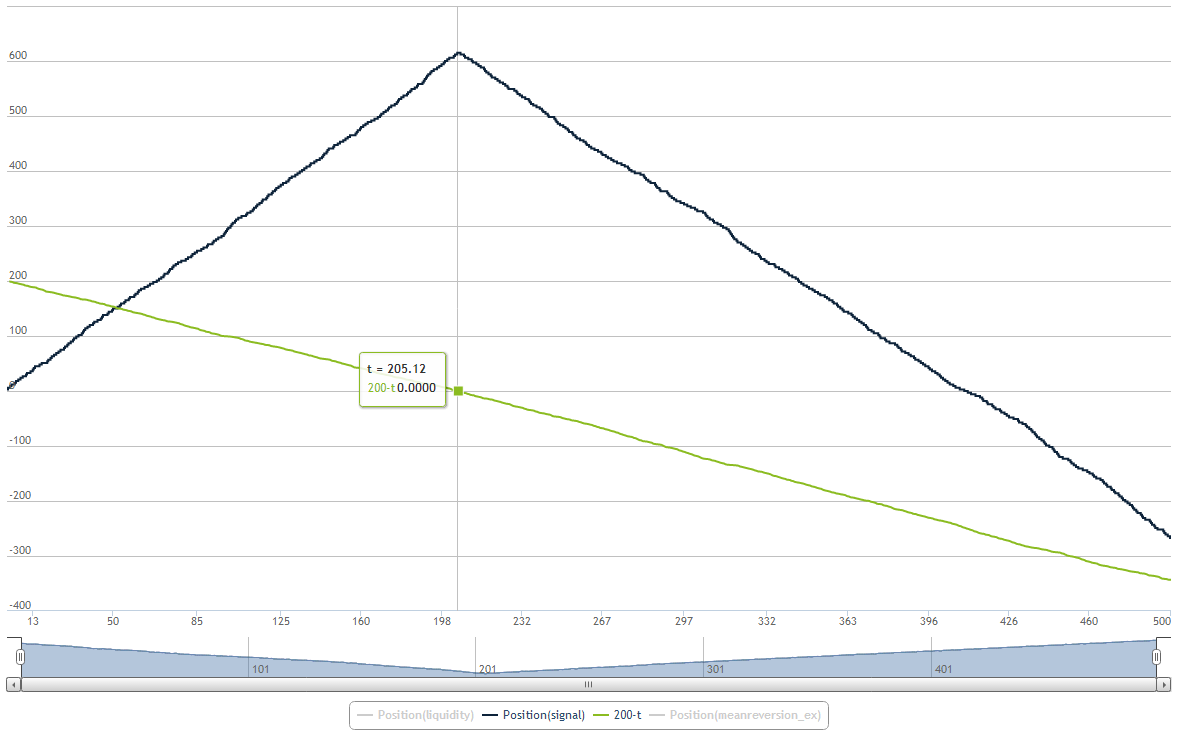
\includegraphics[width=1\linewidth]{Figures/web/signal.png}}

\subsection{Trend follower}\label{trend-follower}

Trend follower can be considered as a sort of a signal strategy where
the \texttt{signal} is a trend of the asset's price. Under trend we
understand the first derivative of some moving average. If the
derivative is positive, the trader buys; if the derivative is negative,
it sells. Since a moving average is a continuously changing signal, we
check its derivative at moments of time given by \texttt{eventGen}.

\begin{verbatim}
type TrendFollower(
        /** parameter |alpha| for exponentially weighted moving average */
        alpha   = 0.15,
        /** threshold when the trader starts to act */
        threshold    = 0.0,
        /** asset in question */
        book = .orderbook.OfTrader()) : SignalStrategy
{
    def Signal_Value
             =  book~>MidPrice
                    ~>EW(alpha)~>Avg
                    ~>Derivative
}
\end{verbatim}


\centerline{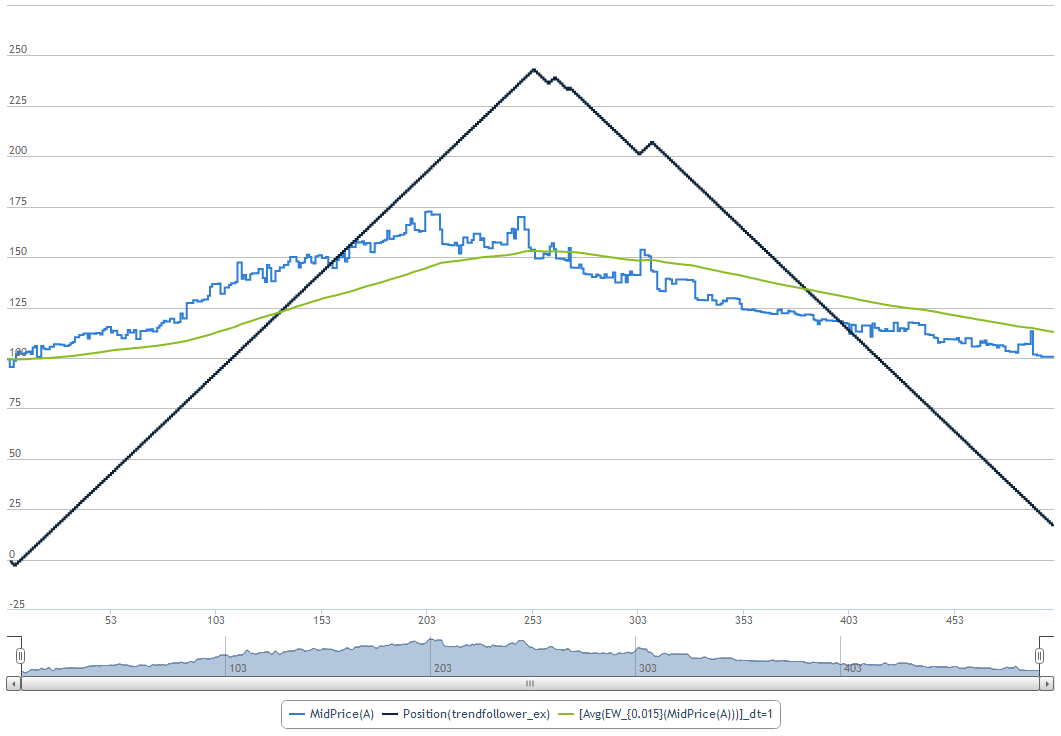
\includegraphics[width=1\linewidth]{Figures/web/trendfollower.png}}

\subsection{Crossing averages
strategy}\label{crossing-averages-strategy}

Crossing averages strategy can be considered as a sort of a signal
strategy where the \texttt{signal} is a difference between two moving
averages of the asset's price.

\begin{verbatim}
type CrossingAverages(
        /** parameter |alpha| for exponentially weighted moving average 1 */
        alpha_1 = 0.15,
        /** parameter |alpha| for exponentially weighted moving average 2 */
        alpha_2 = 0.015,
        /** threshold when the trader starts to act */
        threshold    = 0.0,
        /** asset in question */
        book = .orderbook.OfTrader()) : SignalStrategy
{
    def Signal_Value =  book~>MidPrice~>EW(alpha_1)~>Avg -
                        book~>MidPrice~>EW(alpha_2)~>Avg
}
\end{verbatim}

\centerline{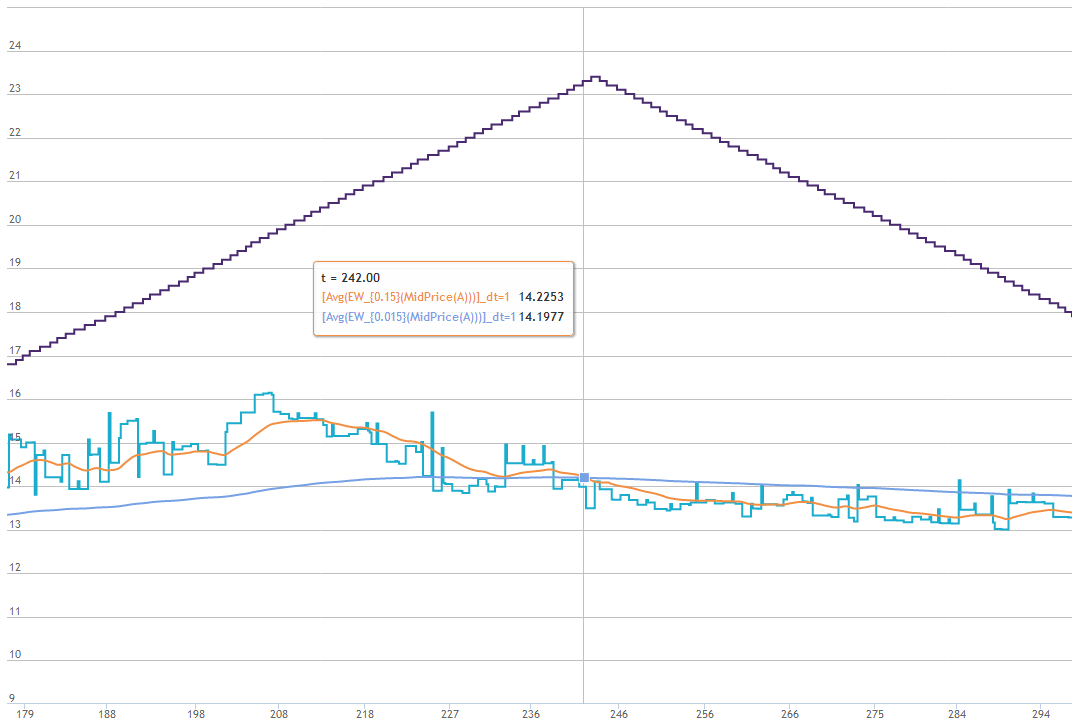
\includegraphics[width=1\linewidth]{Figures/web/twoaverages.png}}

\subsection{Fundamental value
strategy}\label{fundamental-value-strategy}

Fundamental value strategy believes that an asset should cost some
specific price (\texttt{fundamental value}) and if current asset price
is lower than the fundamental value it starts to buy the asset and if
the price is higher than the fundamental value it starts to sell the
asset.

\begin{verbatim}
abstract type FundamentalValueStrategy() : SideStrategy
{
    def book = .orderbook.OfTrader()

    def Side
        =   if book~>Bids~>BestPrice > Fundamental_Value then side.Sell() else
            if book~>Asks~>BestPrice < Fundamental_Value then side.Buy()  else
                                                              side.Nothing()
}

type FundamentalValue(/** observable fundamental value */
                      fv = .constant(200.)) : FundamentalValueStrategy
{
    def Fundamental_Value = fv
}
\end{verbatim}

\centerline{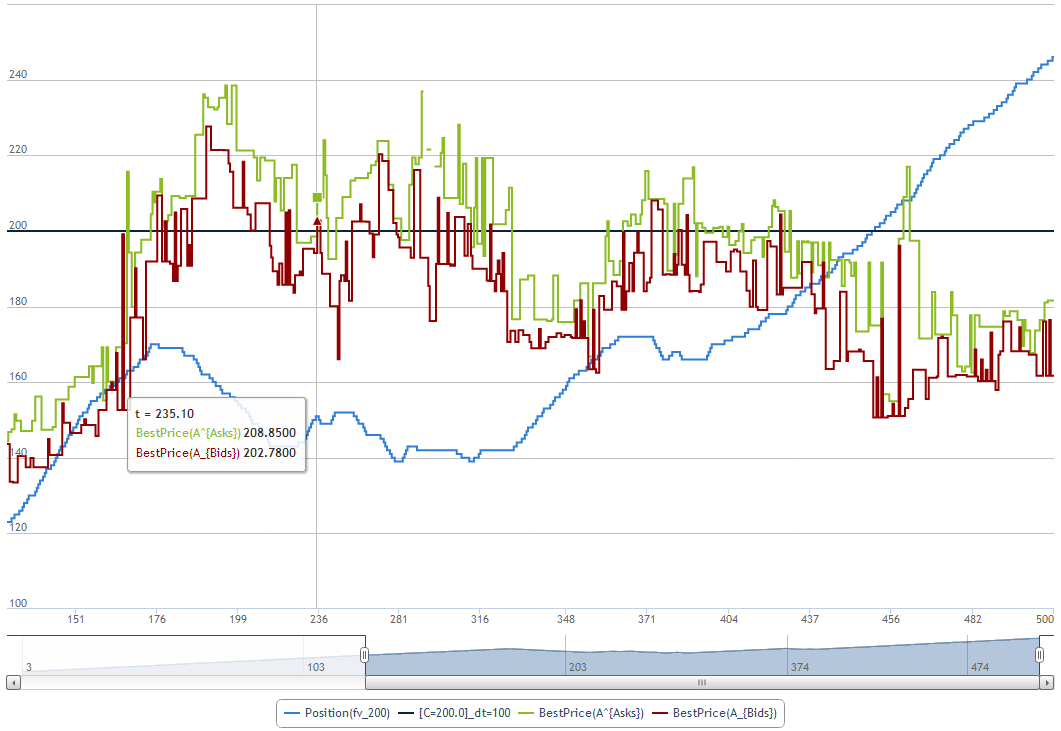
\includegraphics[width=1\linewidth]{Figures/web/fundamentalvalue.png}}

\subsection{Mean reverting strategy}\label{mean-reverting-strategy}

Mean reverting strategy is a kind of a fundamental value strategy with
\texttt{fundamentalValue} equal to a moving average of the asset's
price.

\begin{verbatim}
type MeanReversion(alpha = 0.15) : FundamentalValueStrategy
{
    def Fundamental_Value = book~>MidPrice~>EW(alpha)~>Avg
}
\end{verbatim}

\centerline{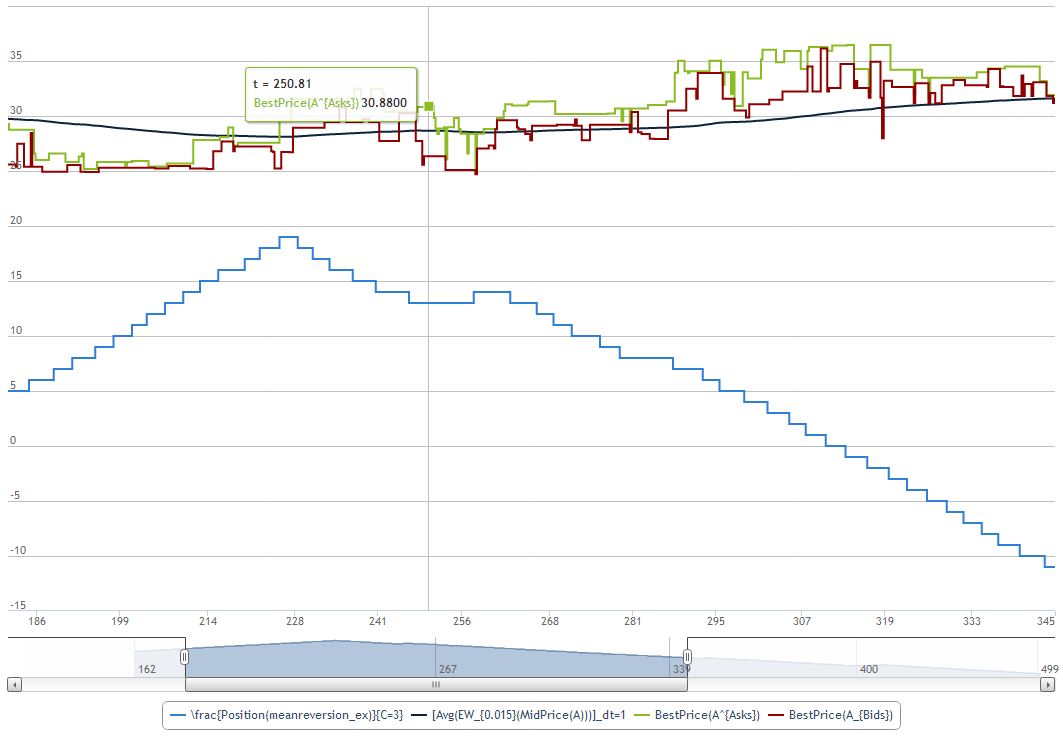
\includegraphics[width=1\linewidth]{Figures/web/meanreversion.png}}

\subsection{Dependency trading
strategy}\label{dependency-trading-strategy}

Dependent price strategy believes that the fair price of an asset
\texttt{A} is completely correlated with price of another asset
\texttt{B} and the following relation should be held:
\texttt{Price(A) = k*Price(B)}, where \texttt{k} is some factor. It may
be considered as a variety of a fundamental value strategy.

\begin{verbatim}
type PairTrading(
        /** reference to order book for another asset
          * used to evaluate fair price of our asset */
        bookToDependOn  = .orderbook.OfTrader(),
        /** multiplier to obtain fair asset price from the reference asset price */
        factor          = 1.0) : FundamentalValueStrategy
{
    def Fundamental_Value = bookToDependOn~>MidPrice * factor
}
\end{verbatim}

\centerline{\includegraphics[width=1\linewidth]{Figures/web/dependency.png}}

\subsection{Desired position
strategies}\label{desired-position-strategies}

These strategies keep track of the trader's position (actual position +
pending orders volume) and if \texttt{desiredVolume} changes it creates
orders in order to cover the gap between the current and the desired
position.

\begin{verbatim}
abstract type DesiredPositionStrategy
{
    def Position = 
        DesiredPosition - trader~>Position - trader~>PendingVolume

    def Strategy(orderFactory = order.signedVolume.MarketSigned()) =
    
        (orderFactory(Position))~>Strategy
}
\end{verbatim}

\subsection{Bollinger bands strategy}\label{bollinger-bands-strategy}

Bollinger band strategy believes that a trader should take a position
equal to the difference between the current asset price and its average
divided on its standard deviation (and scaled by some \texttt{factor}).

\begin{verbatim}
type Bollinger_linear(
            /** alpha parameter for exponentially weighted
              * moving everage and variance */
            alpha   = 0.15,
            /** observable scaling function that maps
              * relative deviation to desired position */
            k       = .const(0.5),
            /** trader in question */
            trader  = .trader.SingleProxy()) : DesiredPositionStrategy
{
    def DesiredPosition = trader~>Orderbook~>MidPrice
                                           ~>EW(alpha)~>RelStdDev
                                           ~>OnEveryDt(1.0) * k
}
\end{verbatim}

\subsection{Relative Strength Index
strategy}\label{relative-strength-index-strategy}

Relative Strength Index strategy believes that a trader should take a
position equal to deviation of its relative strength index from 50
scaled by some \texttt{factor}.

\begin{verbatim}
type RSI_linear(
        /** alpha parameter for exponentially moving averages of 
          * up movements and down movements */
        alpha = 1./14.,
        /** observable scaling function that maps RSI deviation 
          * from 50 to the desired position */
        k = .const(-0.04),
        /** lag for calculating up and down movements */
        timeframe = 1.,
        /** trader in question */
        trader = .trader.SingleProxy()) : DesiredPositionStrategy
{
    def DesiredPosition = (50. - 
        trader~>Orderbook
              ~>MidPrice
              ~>RSI(timeframe, alpha)~>Value
              ~>OnEveryDt(1.0)) * k
}
\end{verbatim}

\subsection{Market data strategy}\label{market-data-strategy}

This strategy allows to drive the asset price based on historical market
data by creating large volume orders for the given price. Every time
step of 1 time unit in the simulation corresponds to a 1 day in the
market data. At each time step the previous Limit Buy/Sell orders are
cancelled and new ones are created based on the next price of the market
data.

It is implemented as a strategy that wakes up once and create a
composition of iceberg and floating price orders. The floating price is
equal to the current quote plus/minus some delta and the iceberg order
breaks an `infinite' limit order into small lots.

\section{Adaptive strategies}\label{adaptive-strategies}

Adaptive strategies aggregate one or several other strategies and
control their execution (e.g. suspending/resuming it) depending on some
factors (e.g. efficiency estimation).

Class \texttt{strategy.Suspendable(strategy, predicate)} wraps
\texttt{strategy} and passes its orders further only if the observable
\texttt{predicate} evaluates to true.

There are many ways to estimate a strategy efficiency. First, we need to
associate with a strategy some kind of an account to track position and
balance changes induced by the strategy's trades. Second, given an
account we may evaluate the strategy's efficiency.

At the moment there are two ways to track strategy position and balance
changes:

\begin{itemize}
\itemsep1pt\parskip0pt\parsep0pt
\item
  \textbf{Virtual market order account}
  (\texttt{strategy.adaptive.VirtualMarket} class) listens orders issued
  by the strategy and for every order makes a request to the orderbook
  in order to estimate impact of trades produced by the order. At the
  moment correct estimation is done only for market orders
  (\texttt{request.EvalMarketOrder} is used) but order impact is
  estimated even if the strategy is suspended.
\item
  \textbf{Actually traded account}
  (\texttt{strategy.adaptive.ActuallyTraded} class) listens to
  \texttt{on\_traded} event of the strategy's trader and collects
  position and balance change produced by orders of this strategy. It
  allows to track impact of orders of any type but doesn't take into
  account orders issued by a suspended strategy.
\end{itemize}

Strategy efficiency can be estimated in different ways:

\begin{itemize}
\itemsep1pt\parskip0pt\parsep0pt
\item
  \textbf{Efficiency}: ``cleared'' trader's balance
  \texttt{eff = observable.Efficiency(}
  \texttt{                    strategy.adaptive.VirtualMarket(aStrategy))}
\item
  \textbf{Efficiency trend}: first derivative of some moving average of
  the trader's efficiency \texttt{ops.derivative(EWMA(eff, alpha))}
\item
  \textbf{Efficiency movements}: difference between the efficiency and
  its lagged value \texttt{eff - Lagged(eff, timeframe)}
\item
  \textbf{Scoring}: counting positive and negative movements of the
  effiency
\end{itemize}

\subsection{Trade-if-profitable
strategy}\label{trade-if-profitable-strategy}

Suspends an aggregated strategy if its effiency is estimated negatively.
By default, it uses \texttt{strategy.adaptive.VirtualMarket} as strategy
tracking account and efficiency trend as efficiency evaluator:

\begin{verbatim}
TradeIfProfitable(strategy,
                  account  = adaptive.virtualMarket,
                  performance = weight.efficiencyTrend) ::=

    efficiency = performance(account(strategy)) in
    Suspendable(strategy, efficiency >= 0)
\end{verbatim}

\centerline{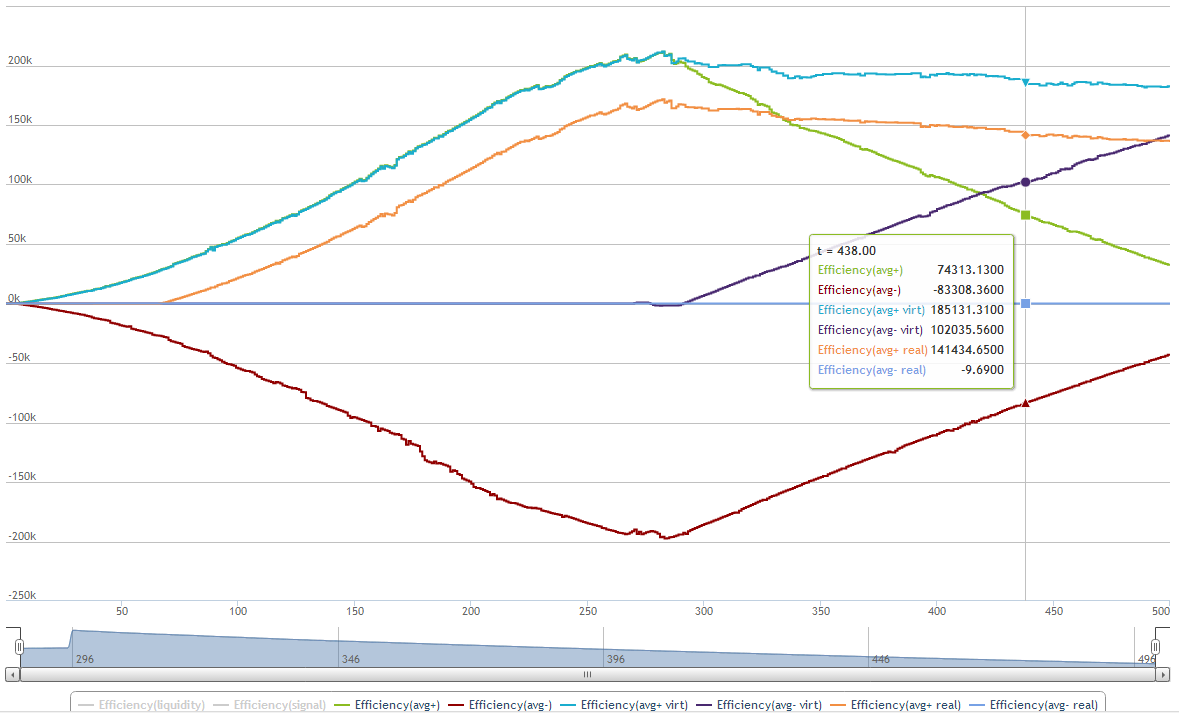
\includegraphics[width=1\linewidth]{Figures/web/tradeifprofitable.png}}

\subsection{Choose-the-best strategy}\label{choose-the-best-strategy}

This strategy aggregates an array of strategies and estimates their
efficiencies. At some moments of time it chooses a strategy with the
best performance and suspends others.

\centerline{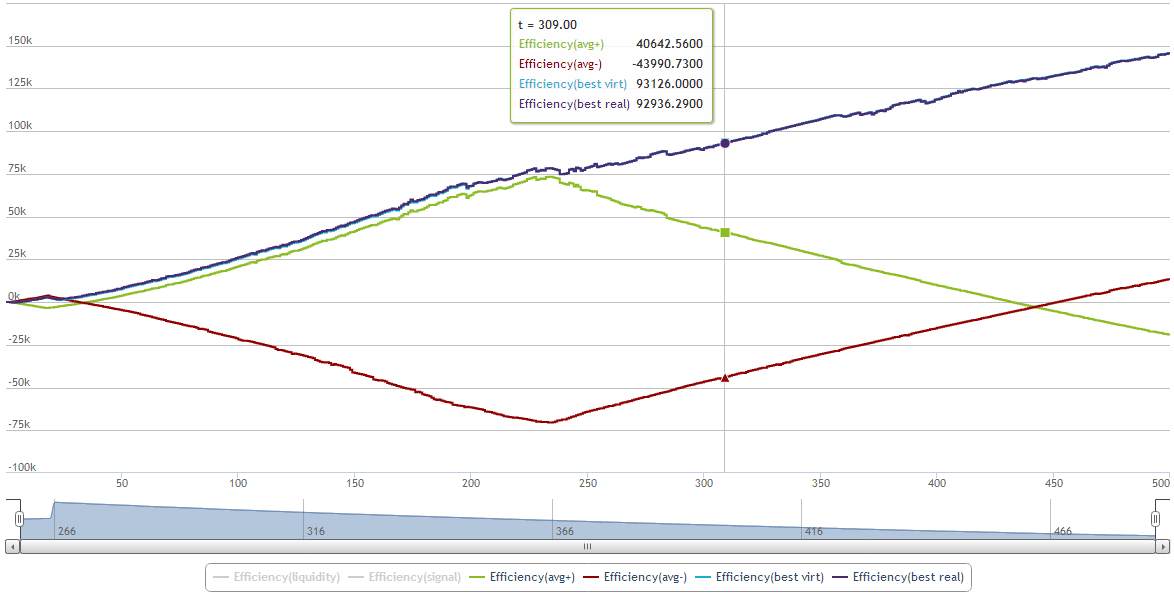
\includegraphics[width=1\linewidth]{Figures/web/choosethebest.png}}

\subsection{Multiarmed bandit strategy}\label{multiarmed-bandit-strategy}

This strategy stores a weight for each aggregated strategy and regularly
updates it. Then it normilizes somehow the weights in order to choose
randomly a strategy. Choose-the-best strategy can be considered as a
particular case of the multiarmed bandit where the weight is equal
performance estimation of a strategy and normalization changes weight of
the best strategy to 1 and weights of other strategies are set to 0.

Multiarmed bandit has following parameters:

\begin{itemize}
\itemsep1pt\parskip0pt\parsep0pt
\item
  \texttt{strategies} -- array of strategies to aggregate
\item
  \texttt{account} -- function that creates an account tracking
  strategy's trades (\texttt{adaptive.VirtualMarket} or
  \texttt{adaptive.ActuallyTraded})
\item
  \texttt{weight} -- function calculating unnormalized weight of a
  strategy (like in trade-if-profitable or choose-the-best strategies)
\item
  \texttt{normalizer} -- function that transforms unnormalized weight
  (for example, to suit a certain range)
\item
  \texttt{corrector} -- function that takes an array of weights and
  makes their sum equal to 1
\end{itemize}

In the following figure efficiency of multiarmed bandit
strategies with different combination of these parameters are shown

\centerline{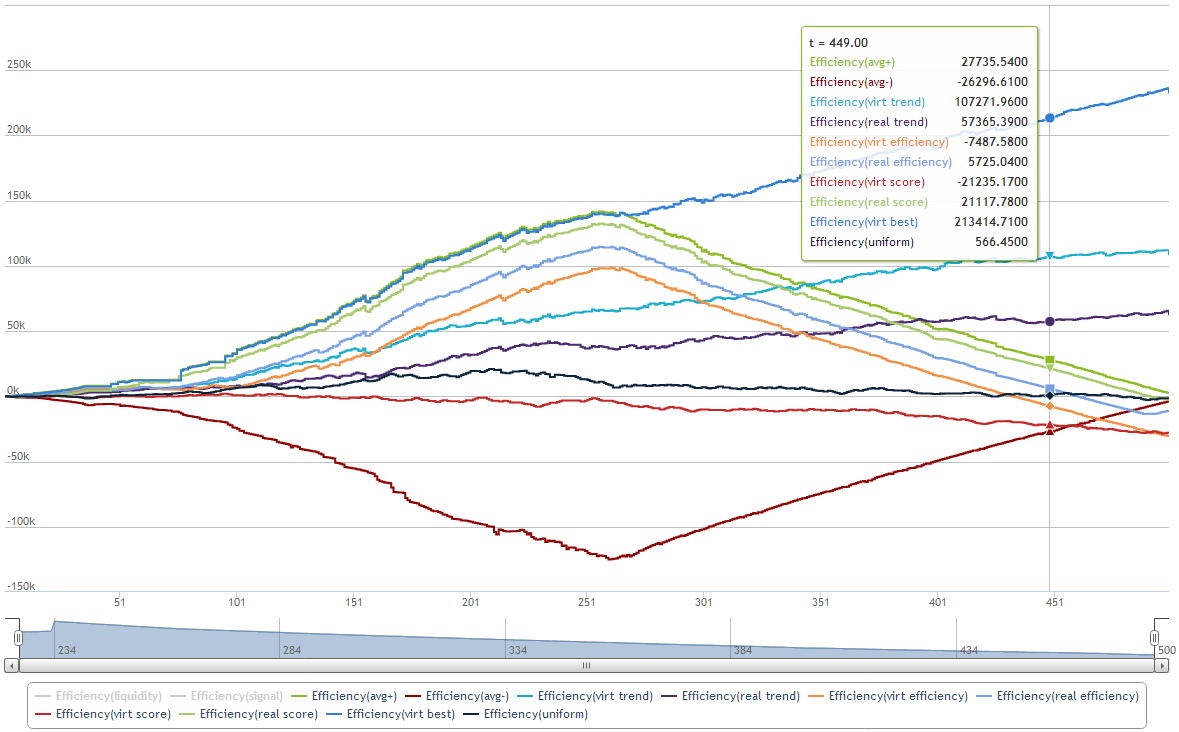
\includegraphics[width=1\linewidth]{talks/multiarmedbandit.png}}

\end{document}





